\chapter{Implementation and Results}
\label{chap:implementation-and-results}

Simulating and solving for the same parameters, we can compare the radial distribution histogram of the simulation output with the obtained, radially-symmetric, equilibrium distribution $\rho \in \functionspace$, cf. \Cref{fig:simulation-solver-comparison}.

% TODO: describe how we find the minimum potential and export in C++

\begin{figure}[H]
  \centering
  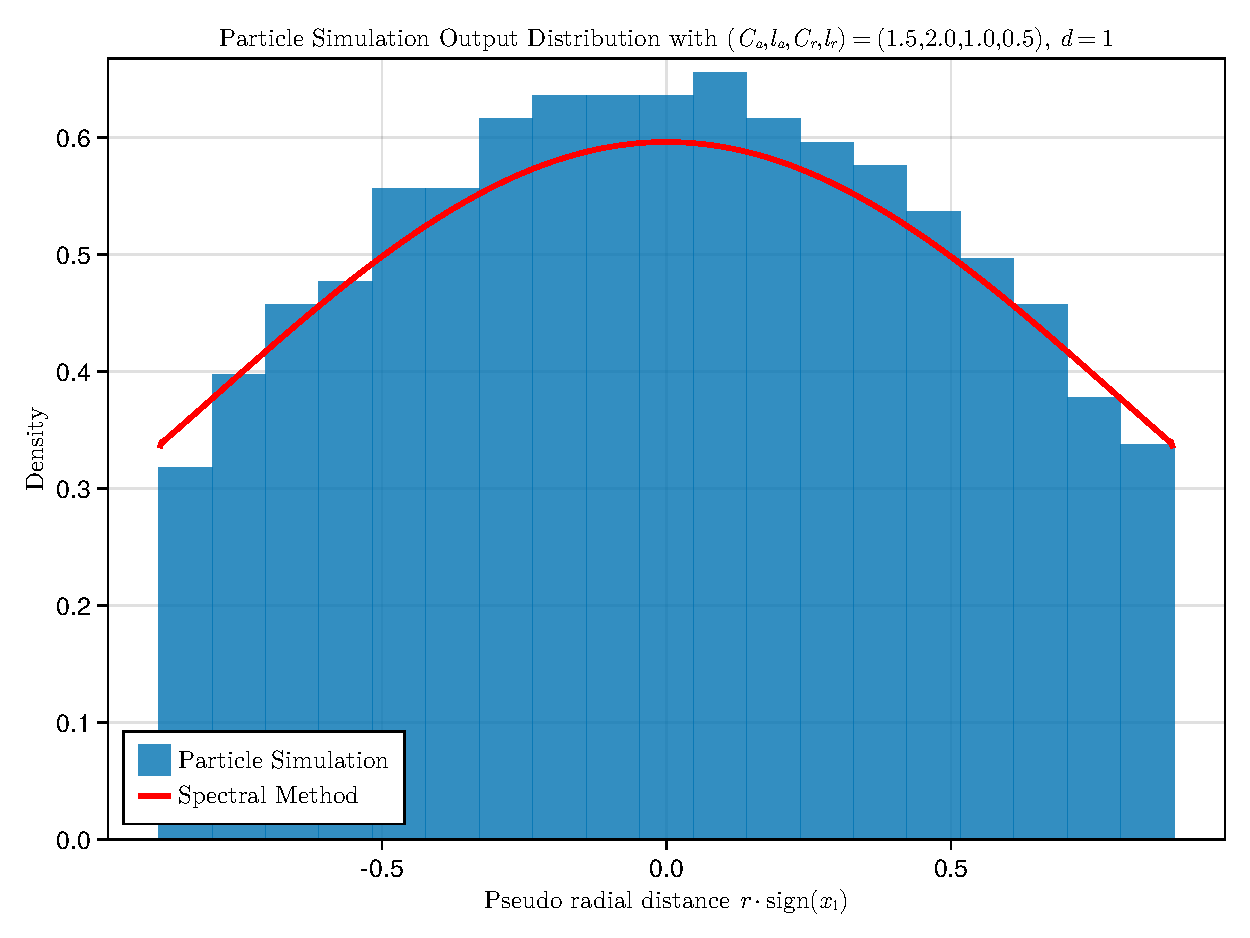
\includegraphics[width=0.8\linewidth]{results/morse/simulation-solver-comparison.pdf}
  \caption[Comparison of histogram and spectral method solution]{Comparison of the radial distance histogram from the simulation output with the $G = 8$ general kernel solvers' equilibrium measure $\rho_{12}(r)$ at $R$ given by the simulator, so without using the outer optimisation routine. The interaction potential in this example is $K(r) = K_{C_a, l_a, C_r, l_r}(r)$ with parameters given above.}
  \label{fig:simulation-solver-comparison}
  % for now
\end{figure}

\section{Further Discussion}
\subsection{Well-Conditionedness}
A common flaw of spectral collocation methods, one could think of them as the highest-order limit of finite difference schemes, is their bad conditioning behaviour.
% TODO: reference

Ideally, we would like the condition number $\kappa(Q)$ to be independent of the order $N$ to which we solve our problem. That means we want
$$\kappa(Q) := \frac{\sigma_{\rm max}(Q)}{\sigma_{\rm min}(Q)} = \frac{\norm{Q}}{\norm{Q^{-1}}} = \mathcal{O}(1)$$
and not $\mathcal{O}(N)$ or even higher orders.

\begin{figure}[H]
  \centering
  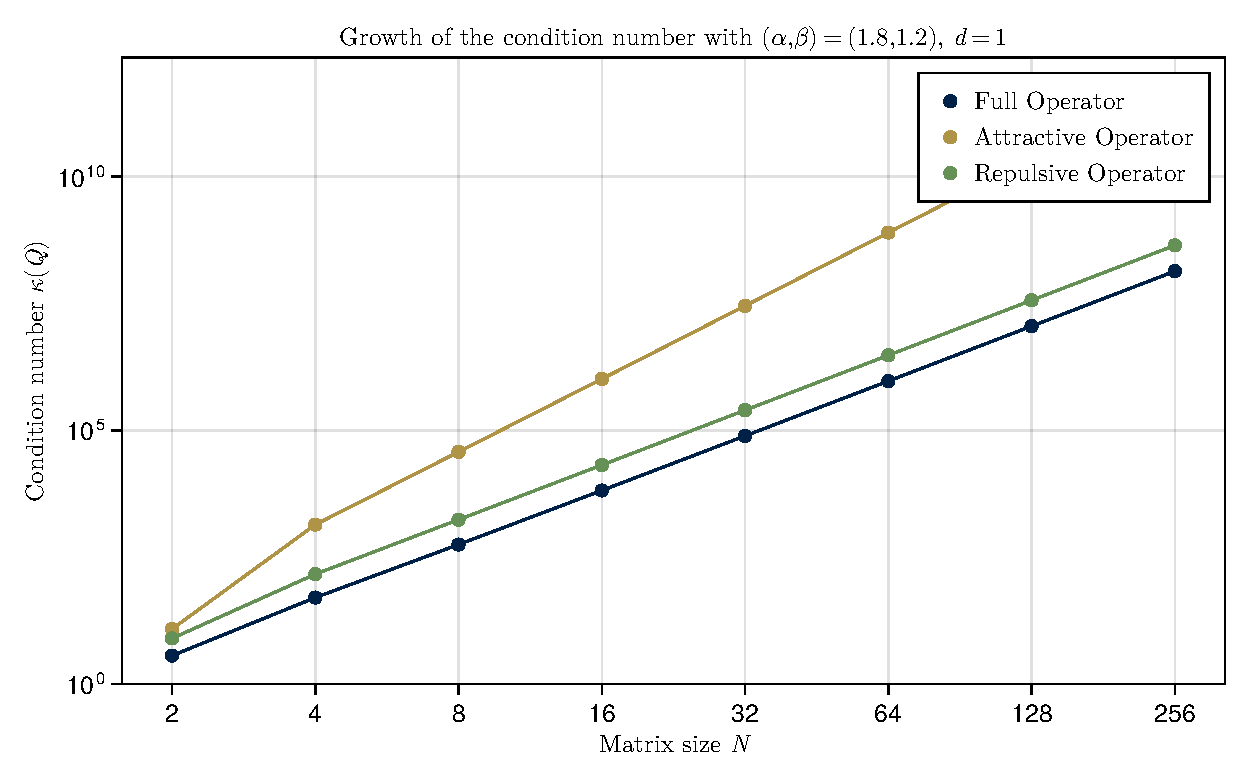
\includegraphics[width=0.8\linewidth]{results/attrep/condition-number-growth.pdf}
  \caption[Growth of the condition number]{Growth of the 2-norm condition number $\kappa(Q)$ of the attractive-repulsive operators $Q^{(\alpha)}$, $Q^{(\beta)}$ and $Q_{\alpha,\beta}$ for growing system size $N$.}
  \label{fig:condition-number-growth}
\end{figure}

\begin{figure}[H]
  \centering
  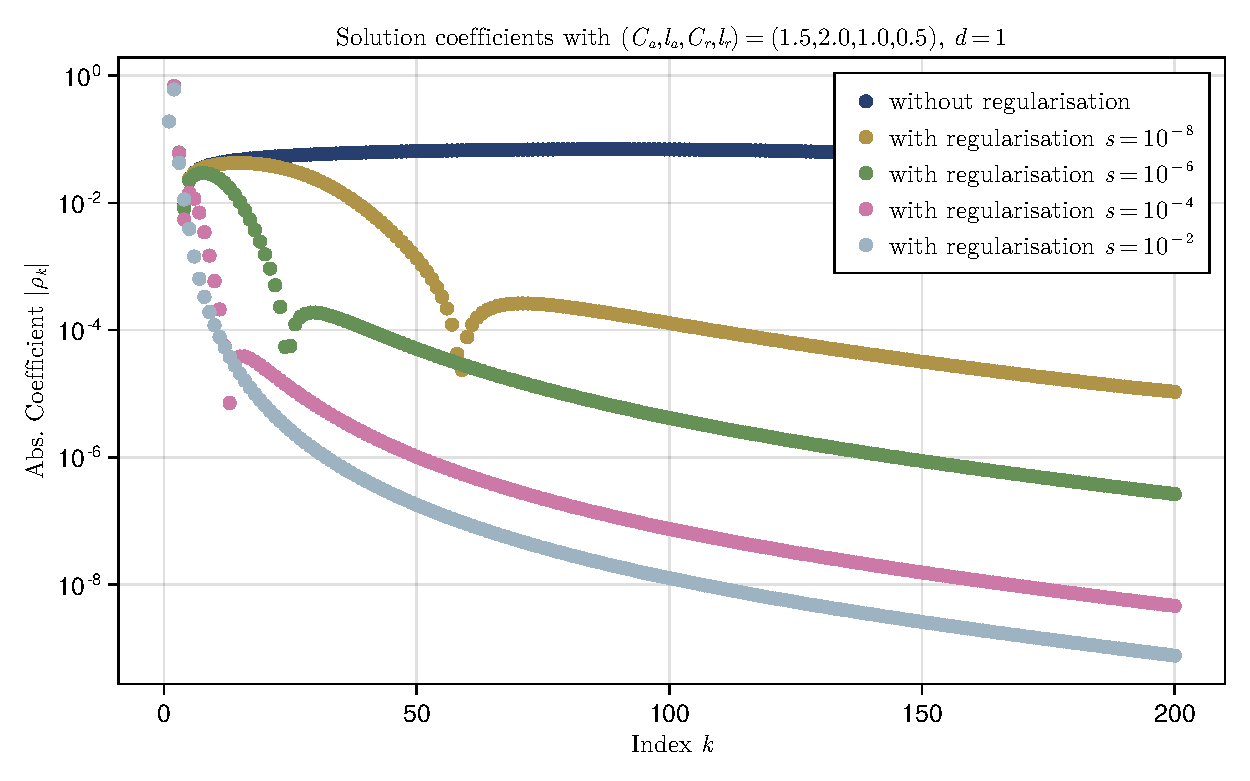
\includegraphics[width=0.8\linewidth]{results/morse/coefficients.pdf}
  \caption[Absolute value of the coefficients with and without regularisation]{Absolute value of the solution coefficients $\rho_k$ with and without Tikhonov regularisation after the solution of a $200 \times 200$ linear system.}
  \label{fig:coefficients}
\end{figure}

\section{Implementation Architecture}
The spectral method solver is written in Julia \parencite{2017-julia} whereas the simulator is written in C++.

To compile the simulator, please run \\
\bashblock{conan install . ----output-folder=build ----build=missing} \\
\bashblock{cd build; cmake .. -DCMAKE\_BUILD\_TYPE=Release} \\
\bashblock{make -j4}
in a bash terminal.

In order to run tests of the numerical solver implementation, run \\
\bashblock{julia solver/tests.jl} \\
in a bash terminal. In order to regenerate all plots at once, including simulation output from the C++ implementation, run \\
\bashblock{julia solver/plotall.jl} \\
in a terminal.
% \hierKoennteIhreWerbungStehen

\section{Runtime Analysis}
\label{sec:runtime-analysis}
The following benchmarks were accumulated on an Intel\textregistered \, i7-5600U CPU running at \SI{2.6}{\giga\hertz} as the average over 3 individual runs with different test vectors, consistent across different parameter runs.
% \hierKoennteIhreWerbungStehen
